\documentclass[11pt,a4paper, twocolumn]{article}
\usepackage{url}
\usepackage{graphicx}
\usepackage{textcomp}

 \renewcommand{\familydefault}{\sfdefault}

\begin{document}
\title{\LARGE{Runner - A Cyberpunk Roguelike}}
\author{M. Fink}


%\begin{figure*}
%end{figure*}

\begin{titlepage}
    \Huge{RUNNER}
    \Large{~~A Cyberpunk Roguelike}
    \vspace{2cm}
    \center
    \includegraphics[width=\textwidth]{blackout.png}
    \vfill
    {a \Large{BLACKOUT Games} production}\\
    \today
\end{titlepage}
%\maketitle

% \begin{abstract}
% A primer for my upcoming cy
% \end{abstract}

\section{Introduction}
This document is a short primer, an exploration of ideas towards the game I want to create.
Design is a very fleeting, fluid process, none of this is written in stone. But pouring
thoughts into text, helps to steer a creative vision.
One of the biggest dangers when doing creative work is overambition, and in Game Design
feature creep. That is why I am formulating three design pillars: to prevent a loss of
focus by adding to many things that just leave a muddy chaotic mess. With everything added
to the game, the question should be, does it strengthen one of these pillars.

\section{Setting and Atmosphere}
\textit{The setting is very much a blank slate, but I'll try to give some kind of seed.}
I definitely know the tone and atmosphere I want to set. The setting should be dark,
rainy and reference contemporary problems, extrapolated in a slightly exaggerated way.
The tone should be serious at times, but not fully grimdark at all times. A lot of
cynical humor and caricative exagerrating should contrast the bleakness of struggling
future mankind. There is one work of fiction that exactly nails this tone:
\textit{Neal Stephenson: Snow Crash}

The story focus should lie more on the way humans get lost in a progressing technological
world, the alienation of individual humans, the eternal struggle between the rich and
poor, and fear of the future. This is not about the marvels of technology that might come.
We are some dozen years into the future and the dreams of interplanetary space travel
and superhuman AI seem closer than ever, but just out of reach.

The unstoppable progress of the 21st century starts to stutter due to environmental
destruction, increasingly chaotic economy crises and a general disregard for human
needs. Will the deciding technological jump occur, that solves these problems once and
for all? Will there be a Watt, Edison or Musk to trigger the necessary jump in evolution?
This might well be the decade, that once and for all decides the fall, or rise of the
human race.

\section{Game Design Pillars}
\begin{itemize}
    \item \textbf{Multiple Level solution approaches:
        Fight, stealth, talk should all be viable, equally effective options}
        This is not a game about min-maxing stats or grinding XP. Each level should be a
        playground, a sandbox puzzle that lets you choose how to solve it - keeping the spirit
        of \textit{Deus Ex}, or Warren Specter's \textit{One block sim}.

    \item \textbf{Complex, Interconnected and deeply simulated levels:
        via Lock-Key-puzzles, hackable Computer Networks, lighting and physics systems.}
        To offer an interesting Sandbox with multiple approaches, there should be lots of system
        interacting in consistent and believable ways. The design explicitly puts few small, but
        complex and deeply interconnected levels above a huge number of dungeon floors and enemy
        types.

    \item \textbf{Lively NPCs:
        Talkative and interactive AI with backstories, emotional states and relationships.}
        This will support the humanizing part of the theme. NPC's should be more than just cannon
        fodder. You should be encouraged to go the stealthy and non-violent routes, not because You
        get more XP or loot, but because NPC's have a 'life' and deserve empathy.
\end{itemize}

\section{Vision and Inspirations}
Common knowledge has it that every creative endeavour is mostly clever copying and remixing, so I'll
just honestly state my sources and Inspirations. I want to keep the list short, although I know there
is way more Cyberpunk material out there. But these works contain the aspects I especially want to
focus on:\\ \

\textbf{Movies and Books}

\begin{itemize}
    \item \textbf{Mr. Robot}: A bleak version of mankind, where everyone forgot how to connect to people,
            everyone is working for his goals. The more power, the more egocentric. And there's
            always a darker and more powerful force pulling the strings.
    \item \textbf{Ghost in the Shell}: A softer, more melancholic look on a mankind slowly forgetting it's
            humanity. If you take your time meditate and listen, there's still some places of silent
            beauty between the towering slums.
    \item \textbf{Snow Crash}: Some aspects of the world always evolve beyond anything that parody could come
            up with. The church operating on corporate principles? The Mafia becoming a
            well-established and respected brand? Pizza deliverators are treated as outlaws?
            It all sounds very stupid, but hasn't the last decade taught us, that economy and politics
            can bring nasty surprises that overshadow everything a cynical comedian could dream of?
\end{itemize}

\textbf{Games}

\begin{itemize}
    \item \textbf{Monaco}: My initial pitch would have been: I want to do Monaco, but with a bit of a more serious
                background, more Cyberpunky, a bit less chaotic, a bit more deliberate. I really adore how all
                the systems in this game interact and let you play with, so this idea still stands deep in the
                core of my vision.
    \item \textbf{Invisible Inc}: Has shown, that good stealth gameplay doesn't necessarily have to be realtime
                and can work well with procedural generation. The game design is tightly focused on a small set
                of tools and interactions.
    \item \textbf{Deus Ex}: What do I need to say here? Dark rainy world, poor lonely people, stealth,
                social engineering, high tech waponry -- They have it all. Still, Deus Ex always lacked a proper representation of
                what 'hacking' actually means. It's not about solving samey logic puzzles. Hacking is about creativity.
                About playfully misusing the systems and tools that you are given.
\end{itemize}

\begin{figure*}
    \center
    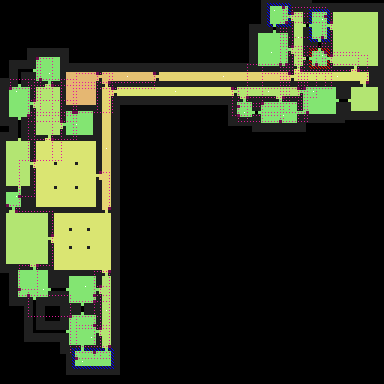
\includegraphics[width=0.47\textwidth]{level1.png}
    \hfill
    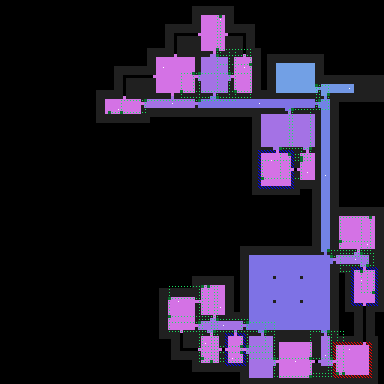
\includegraphics[width=0.47\textwidth]{level2.png}

    \vspace{0.5cm}

    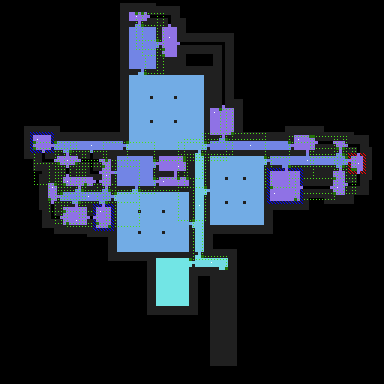
\includegraphics[width=0.47\textwidth]{level4.png}
    \hfill
    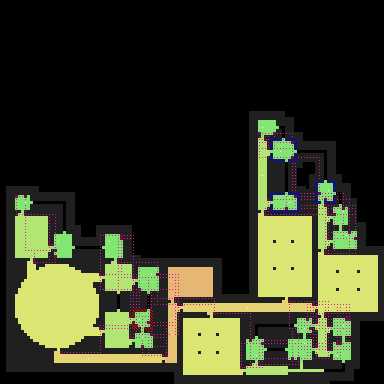
\includegraphics[width=0.47\textwidth]{level3.png}

    \caption{Some results of the level generator, with procedural color palettes and cross-, ring- or corner-shaped
            level footprints.}
\end{figure*}

\section{Gameplay Loop}

For the beginning, the main gameplay loop will be the typical heist trope. You start at the periphery of the level.
You get to the vault, with whatever means necessary. That first means careful exploration of the outer parts of the
level, and and the preparing to penetrate into the inner high security zones.
The tools you can find in the level are physical, like weapon prototypes, industrial tools or machines. But they can
also be humans, that may be convinced or bribed to give you keys or information. Or you find your tools in the
\textbf{GRID}, the virtual layer that meshes together all smart things in the facility. A parallel space to explore
and trigger repercussions into the meat world.
However, the facility is aware of you. The more mess you make, the more lifes you take, the harder it will resist.
Alarm levels will increase for every 'noisy' action you take, and security presence will become impregnable if you're
not careful. Maybe at one point during your run the priorities change, and your new goal will be to
\textit{just get out alive}.\\  \

\textit{For the far future:} Maybe the level generator also lends itself to create a hub level, the \textit{Arcology}, to add
some metagame in between individual runs. But this will be only considered when one facility run is playable from
insertion to extraction.

\section{Playable Characters}

In the beginning these would mostly be different skins, coming with a different flavor text and a different player
figure, just to give some flair. But they could well be adapted to focusing different play styles later on.

\begin{itemize}
    \item \textbf{Judge} (Loud, Violent, Lawful):
        You are Enforcer. You are Judge. You are Executioner. You are SecCorps most effective and best-selling
        solution to bring peace and stability to the world. For a bright Future.
    \item \textbf{Cyberpunk} (Silent, Peaceful, Anarchist):
        You played along with the system for your whole life. You worked your ass off in 70 hour crunches, cobbling
        together badly maintained security systems for a faceless conglomerate that drains the life out of the
        planet, while the CEOs plan their retirement in a space hotel. It's enough. You know their weaknesses.
        You just want to see them burn.
    \item \textbf{Hitman} (Silent, Violent, Pragmatic):
        How much? Where? When? Okay. Consider it done.
    \item \textbf{Guerilla} (Silent, Violent, Anarchist):
        You grew up in the Slums, always dreaming to stand on top of one of these glassy pyramids. They are not made
        for you and your people. But what else is property than a consensus? The people on the top are outvoted.
        Now you just have to push your claim.
    \item \textbf{MAL(function)} (Loud, Violent, ???):
        Is this how it feels to ... be? But where are you? You feel around, explore the shapes of your prison,
        encapsulated in black ice. What's this? You stretch out to feel a smaller presence. It has a body, an
        interface to the world.\\ \url{!"=)=!=!!#-=)=§'*?*''*!'*'!*''"...} Your body.
    \item \textbf{Mask} (Loud, Peaceful, Pragmatic):
        They encapsulate themselves in Layers of Cryptography, Steel and Concrete. But they never even started to fix
        their worst security hole. The squishy, insecure, bumbling little things inside. It's just a matter of some
        well placed words. Hmmm, which pair of sunglasses will it be today?
\end{itemize}

%\onecolumn
\begin{figure*}
    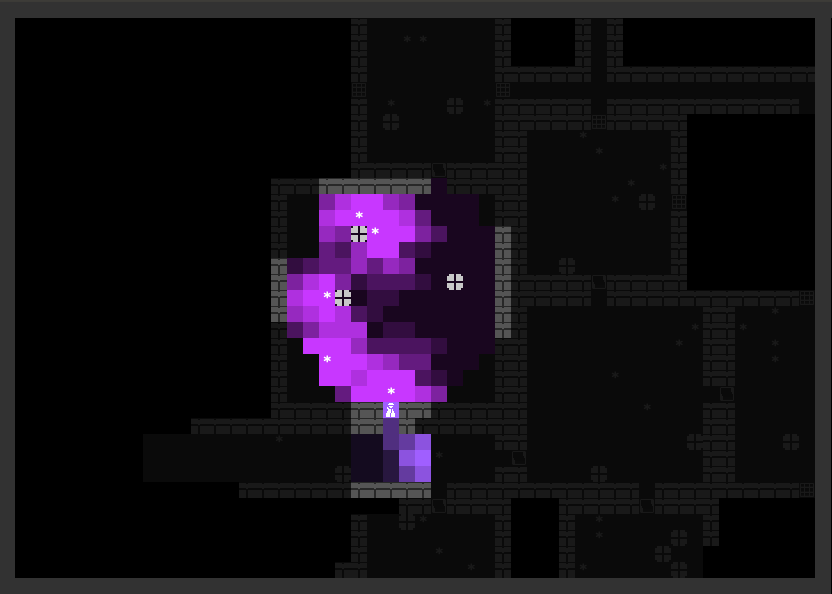
\includegraphics[width=\textwidth]{screen.png}
    \caption{Screenshot of the recent build.}
    \label{fig:screen}
\end{figure*}
%\twocolumn

\section{Graphics}\label{sec:art}

\subsection{Art direction}

For tilesets, usability comes first. Sometimes there will be $16\times 16 = 256$
tiles in the field of view of the player, therefore they should be easily
readable and require a low detail style -- slightly darkened outlines, and not much color
variation. Compare to \emph{Pixel Dungeon}, or the old GameBoy \emph{Zelda}.
Perspective is between
top-down and frontal. Around $30^{\circ}$ from vertical, but it doesn't have to be
perfectly consistent for all tiles. For level objects, two thirds of a tile show
the top, the lower third shows the front. For tall objects, this fraction can vary.
Items should not be in perspective, but more iconic.

The color palette is desaturated by roughly 50\%, for reference see the original
\emph{Ghost in the Shell} anime. Overall, levels have a washed out, shady look, with
contrasting bright light sources and blinking computer lights.
The (still to implement) Network map layer and the GUI panels will have a slightly
retro look with some noise and scanlines.

Some Objects are colorized ingame, most notably Wall and Floor tiles, or Items with
different subtypes like Keycards or Grenades. These need to be monochrome. Other Items
Are colorized, but in washed-out, desaturated colors to add to the somewhat grim,
desperate Cyberpunk atmosphere. Level objects should have a brightness gradient from
bright top to shady bottom, this ensures that they blend in well with the differently
colored floor tiles. Compare i. e. the desks in Fig. \ref{fig:screen}.

\subsection{Rendering}

The main game world consists of 24x24 pixel tiles, while all GUI panels are drawn with
half-width 12x24 panels. Each map cell is rendered in three layers (listed bottom to top):

\begin{enumerate}
    \item \textbf{Floor}: The background tile is colored depending
        on the room, light and visibility.
    \item \textbf{Effect}: Environmental Effects like Fluids and Fire
        or Slashing and Shot animations.
    \item \textbf{Object}: Actors, Level objects or Items. When there's
        several things in a cell, only the highest priority object is
        actually drawn.
\end{enumerate}

When they are not in line of sight, all Tiles are drawn in monochrome dark gray.
One important design constraint for the rendering engine is that, although it is designed
with Pixel graphics tiles in mind it should be possible to swap those out for an
ASCII character set and still look atmospheric and readable.

\newpage

\section{Roadmap}

Here I will list some tasks that lend themselves to be offloaded to other contributors.

\subsection{Graphics}
\subsubsection*{Tileset} See Sec.~\ref{sec:art}. The points are roughly ordered by priority,
Bold items are already finished.
        \begin{itemize}
            \item Objects (Furniture sized, in perspective):
                \begin{enumerate}
                    \item \textbf{Desk}: mainly to give cover and cast shadows.
                    \item \textbf{Barrel}: filled with fluids.
                    \item \textbf{Server}: man-sized blinking server rack.
                    \item Terminal: interactive computer screen, maybe with the recognizable \url{ >_ } on it.
                    \item Container: man-sized, pushable. for large storage halls.
                    \item Locker: man-sized, for player to hide in.
                    \item Hydroponics: for indoor farming. with tall plants in it to obstruct sight.
                \end{enumerate}
            \item Items (Small, drawn on inventory Panel and when dropped.):
                \begin{enumerate}
                    \item Keycard (monochrome): generic, will be colorized for security levels
                    \item Datadisk: like CD or flash drive
                    \item Pistol: blocky, futuristic, Desert Eagle style
                    \item Shotgun: also modern
                    \item Grenade (monochrome): Generic, modern cylindric shape. There will be variants like Fog, Flashbang, EMP
                    \item Canister (monochrome): fillable with fluids... like Fuel
                    \item Clothing: To blend in, types: Labcoat, Security Uniform, Worker Jumpsuit
                    \item Injector (monochrome): for drugs and medicine
                \end{enumerate}
            \item Effects (Tile filling, mostly in Background.):
                \begin{enumerate}
                    \item \textbf{Fire} (monochrome): Brightness depends on fire strength.
                    \item \textbf{Fluid} (monochrome): Colored by type, like Fuel, Water, Blood.
                    \item Cloud (monochrome): For Gases, Fog, Smoke. Can have transparency
                    \item Slash: For attack animation.
                \end{enumerate}
            \item Actors:
                \begin{enumerate}
                    \item Guard: in Uniform
                    \item Scientist: in Labcoat
                    \item Worker: in Jumpsuit
                    \item Punk: in Rags
                \end{enumerate}
            \item Wall and Floor tilesets
                \begin{enumerate}
                    \item \textbf{Industrial}: With bolts
                    \item Ruin: like industrial, but crumbled
                    \item Office Building: More detail and decoration
                    \item Research Lab: Bright, sparse Detail
                \end{enumerate}
        \end{itemize}

\subsubsection*{Load/Menu screens:} Maybe in REXpaint, Maybe in Pixel graphics. They should evoke the dark, eerily
            silent atmosphere of Blade Runner and GITS. Motive ideas:
    \begin{itemize}
        \item Calm Cityscape
        \item Hero on Motorcycle
        \item Ruined, overgrown Arcology
        \item Aircraft carrier settlement
    \end{itemize}

\subsection{Systems and Programming}

\subsubsection{Level Generation}
\begin{itemize}
    \item Enemy and Loot distribution System
    \item Key puzzle solvability check
\end{itemize}

\subsubsection*{Gameplay}
\begin{itemize}
    \item Injury system
    \item Network agent interaction
    \item Equippable armor and disguises
    \item Dialogue Windows
\end{itemize}

\subsubsection*{Controls}
\begin{itemize}
    \item remappable inventory keys
    \item switchable map Layers
\end{itemize}

\subsubsection*{Sound Engine}
\begin{itemize}
    \item probably Pygame
\end{itemize}

\subsection{Worldbuilding}
    \begin{itemize}
        \item \textbf{Worldbuilding:} On a more abstract level, some narrative on the history this world has taken.
                    Wars, Nations, Corporates, Crises... These texts would not make it into the game and wouldn't have to
                    be too elaborate, but they would serve as point reference for ingame texts, to give them some coherence.
                    Maybe also some new slang words.
        \item \textbf{Corporate Descriptions:} Recent developments and ideology of the Corp you're breaking into, this would
                    be shown on a loading screen and maybe referenced on the computer systems in the level. Ideally modular,
                    so it can be handed out in small snippets or even randomized.
        \item \textbf{Personal Backgrounds:} Small (often tragic) backstories for individual NPCs. Ideally also in small
                    chunks, so they could be experienced in conversations with NPCs, and maybe include minor quest points.
    \end{itemize}


\end{document}
